\chapter{Grundlagen}
\label{chapter_grundlagen}

Der Kernteil der Arbeit beginnt mit einer Darstellung der Grundlagen. Dieser, in der Regel rein theoretische Abschnitt, beinhaltet Begriffsbestimmungen, Beschreibungen zur Methodik und zum verwendeten Material, zu Hard- und Software sowie Begriffsabgrenzungen und anderweitigen Grundlagen ("`Material und Methode"'), welche zum Verst�ndnis der nachfolgenden Ausf�hrungen notwendig sind.

\section{Formeln}
%
Formeln sind f�r jeden Abschnitt rechtsb�ndig von dieser zu nummerieren, um einen sp�teren Bezug in der Arbeit zu gew�hrleisten. Formeln werden �blicherweise in "`Computer Modern Roman"' (\LaTeX{}-Standard) gesetzt. In diesem Template wird die Formel-Schrift bzw. das Package \texttt{eulervm} verwendet. Abgesetzte Formeln werden in \LaTeX{} durch die 
\emph{equation} Umgebung definiert. Formelausdr�cke innerhalb von Textabschnitten erh�lt man durch \$Formel\$.

\subsection*{Beispiel}
%
Der \emph{Sinus cardinalis} oder sinc-Funktion ist eine mathematische Funktion $f$, welche in nicht-normierter Version als

\begin{equation}
	f(x) := \frac{\sin(x)}{x}
	\label{eq:bsp}
\end{equation}

definiert wird. In der digitalen Signalverarbeitung findet meistens nachfolgende normierte Version $\mathrm{si}(x)$ oder $\mathrm{sinc}(x)$ Anwendung \cite{Gru04}, \cite{WikiSinc}. F�r eine Visualisierung dieser Funktionen siehe Abb.~\ref{Darstellung_Sinc}.

\begin{equation}
	f(x) := \frac{\sin(\pi x)}{\pi x}
	\label{eq:bsp2}
\end{equation}

\section{Abbildungen}
%
Abbildungen sind f�r jeden Abschnitt zu nummerieren und mit einer kurzen Bildunterschrift zu versehen, vgl.~Abb.~\ref{Darstellung_Sinc}. Inhalt des Eintrages ist die Bildunterschrift. Beachten Sie, dass in dieser Vorlage bereits Unterordner zur Aufbewahrung der Grafikdateien angelegt wurden.

Bei Grafiken die von anderen Quellen (Internet, Scans) stammen ist die Quelle in der Bildunterschrift zu deklarieren. Wurde die Grafik modifiziert, dann ist dies durch "`modifiziert nach [Quelle]"' oder mit "`nach [Quelle]"' anzugeben.

F�r korrekte Erstellung von Grafiken f�r die Verwendung mit LaTeX siehe \cite{gockel07}.

\begin{figure}[th]
	%\begin{center}
		 % You don't need a file extension or full path, if ...
		 % ... the file is located in the correct directory (./images/pdf, ./images/png)
		 % ... the file has the correct extension (*.pdf, *.png)
		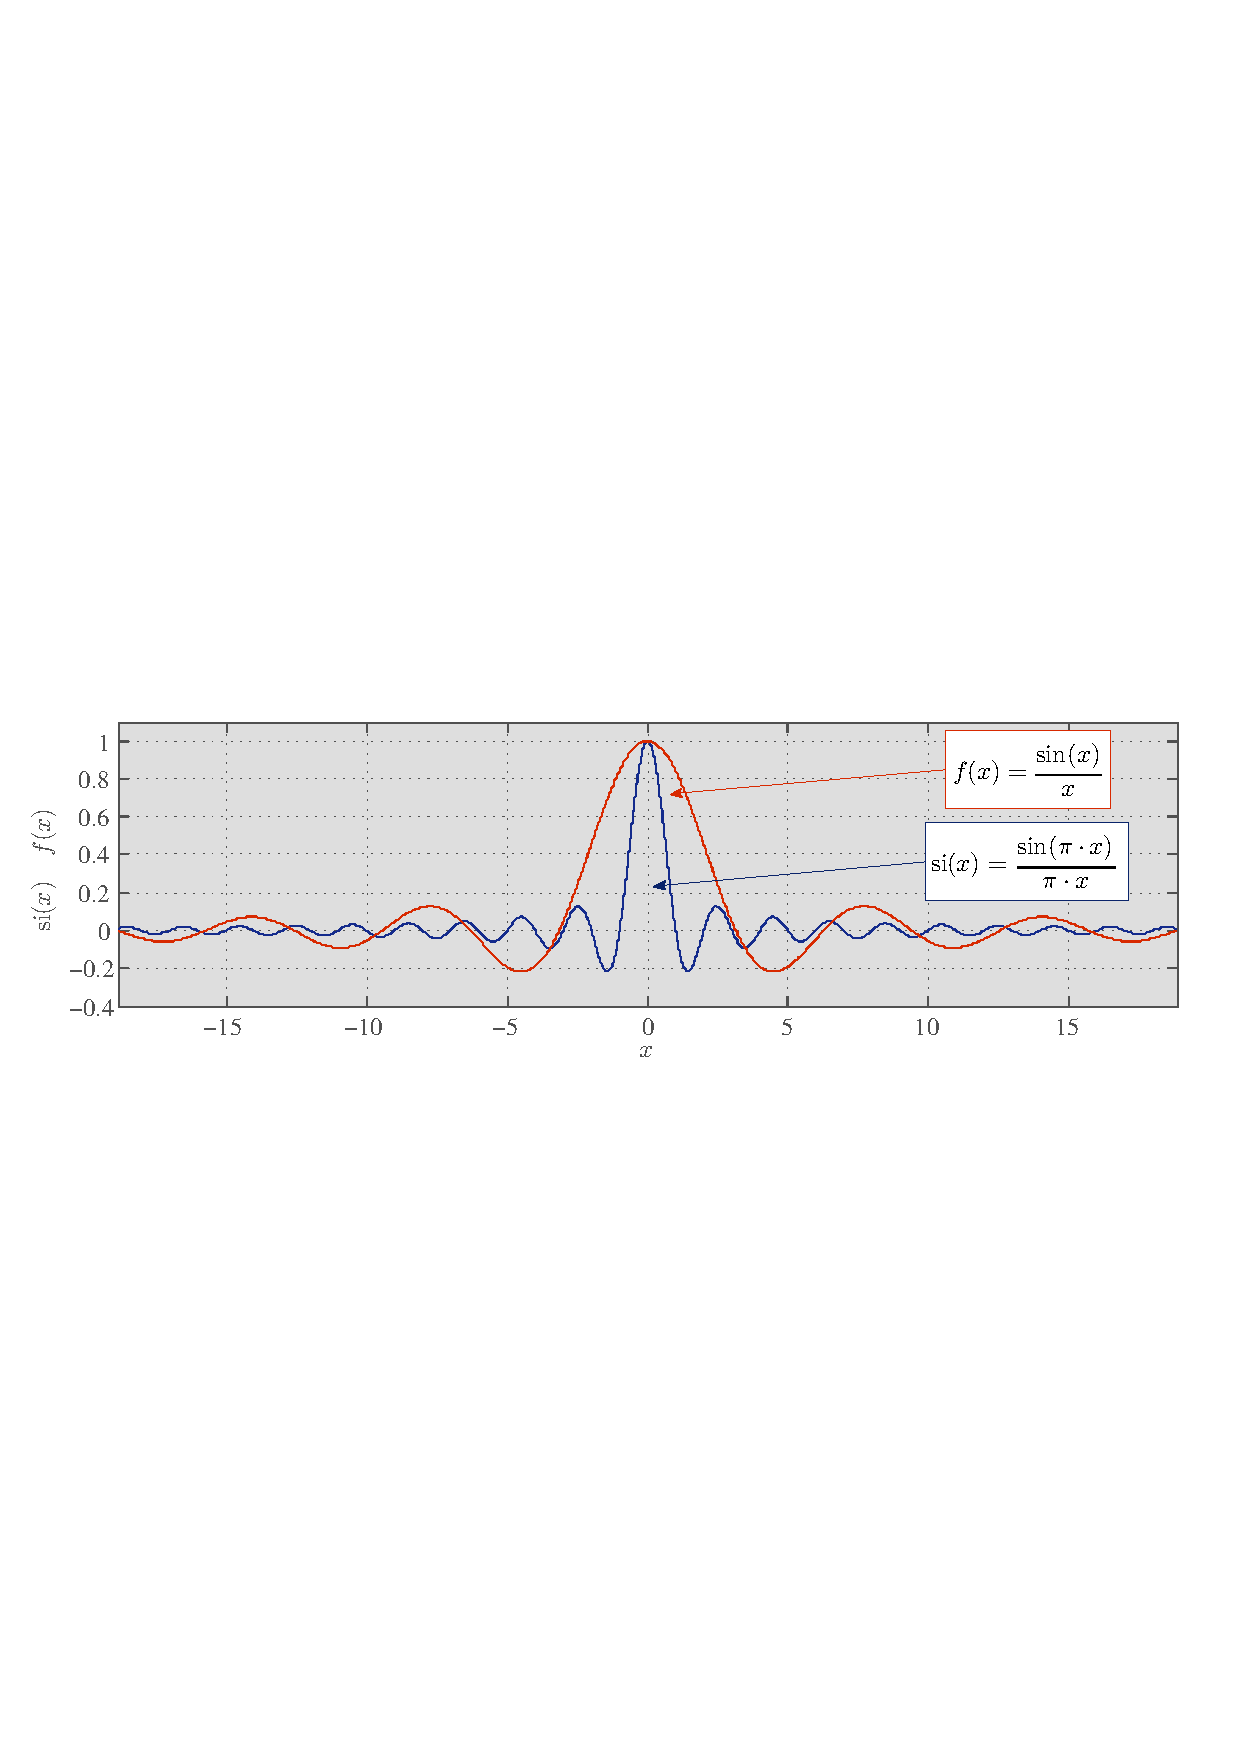
\includegraphics[width=\textwidth]{BilderKapGrundlagen/sincfig}
	%\end{center}
	% Title
	\caption{Darstellung der Sinc-Funktion}
	% Unique name: identifier for referencing
	\label{Darstellung_Sinc}
\end{figure}










%






